\documentclass{article}
\usepackage{graphicx}
\usepackage{listings}
\usepackage{ctex}
\usepackage{graphicx}
\usepackage[a4paper, body={18cm,22cm}]{geometry}
\usepackage{amsmath,amssymb,amstext,wasysym,enumerate,graphicx}
\usepackage{float,abstract,booktabs,indentfirst,amsmath}
\usepackage{array}
\usepackage{booktabs} %调整表格线与上下内容的间隔
\usepackage{multirow}
\usepackage{diagbox}
\usepackage{indentfirst}
\usepackage{bm}
\usepackage{fancyhdr}




\pagestyle{fancy}

\lhead{\bfseries \normalsize 学号:1952033\quad 姓名:侯雅玥 \quad 组员:廖宏 \\实验名称:TTL集成逻辑门参数的测试实验\quad 课程名称:电子技术实验\quad 专业:微电子科学与工程 } 
\rhead{}

\begin{document}
	\section{\zihao{4} 实验名称:TTL集成逻辑门参数的测试实验}
    \section{\zihao{4} 实验目的}
    \zihao {5} (1)了解 TTL.集成逻辑门各参数的意义。\par
               (2)掌握 TTI 集成逻辑门主要参数的测试方法。\par
               (3)掌握 TTl 器件的使用规则。\par

   	\section{\zihao{4} 实验原理}
              
 TTL与非门是目前使用较普遍的一种基本逻辑门电路.
    实验采用74系列双列直插式四-2 输入 TTL 与非门 74LS00 集成芯片进行参数测试,其外形引脚排列及逻辑符号如图1和图2所示。
	\begin{figure}[h]
        \begin{minipage}[t]{0.5\linewidth} % 如果一行放2个图,用0.5,如果3个图,用0.33  
          \centering   
          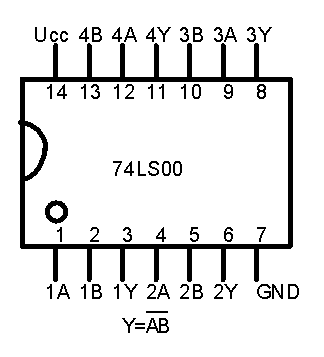
\includegraphics[width=2in]{H:/电子技术试验/4-18/4-18-1.png}   
          \caption{74LS00 外形引脚排列}   
          \label{fig:side:a}   
        \end{minipage}%   
        \begin{minipage}[t]{0.5\linewidth}   
          \centering   
          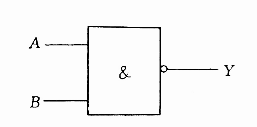
\includegraphics[width=3in]{H:/电子技术试验/4-18/4-18-2png.png}   
          \caption{TTL与非门逻辑符号}   
          \label{fig:side:b}   
        \end{minipage}   
      \end{figure}
               \subsection{平均功耗P}
               TTL逻辑门工作于开态(输出低电平)和关态(输出高电平)时,电源电流值不同。电路处于稳定开态时的空载功耗称为空载导通功耗$P_L$:
             \[P_L=I_{EL}\times U_{CC}\]
               式中,$I_{EL}$是空载导通电源电流;$U_{CC}$是电源电压;\par 
               测试条件:与非门的输入端悬空,输出空载,$U_CC=5V$,如图4所示。电路处于稳定关态时的空载功耗称为空载截止功率$P_H$:
               \[P_H=I_{EH}\times U_{CC}\]
            式中,$I_{EH}$是空载截止电源电压;$U_{CC}$是电源电压\par
            测试条件:与非门的输入端至少有一个接地,输出空载,$U_{CC}=5V$,如图5所示。
            平均功耗:P为电路空载导通功耗$ P_L$ 与空载截止功耗$ P_H$的平均值。即\[P=\frac{P_L+P_H}{2}\]
            \subsection{输入短路电流$I_S$}
            输入短路电流是在输入端接地时流经输入端的电流$ I_{IS}$。 由于输入端接地,因此又称它为低电平输入电流,以 $I_{IL}$表示。
            它是 TTL 集成逻辑门的一个重要参数,因为输入电流就是前级门电路的负载电流,其大小直接影响前级电路带动负载的个数,因此$I_{IL}$越小越好。
            测试条件∶被测某个输入端通过电流表接地,其余各输入端悬空,输出空载, $U_{CC} =5V$,如图 9 所示。

            \subsection{输入短路电流$I_S$}
            (3)电压传输特性
             TTL集成逻辑门电压传输特性是指输出电压$U_o$。随输入电压$U_i$变化的关系曲线∶
          \[U_o=f(U_i)\]
电压传输特性的测试方法可采用逐点测试法,即利用电位器调节被测输入电压 $U_i$,逐点测出对应的输出电压$U_o$,根据测量的结果画出电压传输特性曲线。
电压传输特性曲线可以反映出TTL与非门$U_{oH},U_{oL},U_{on},U_{off}$等主要特性参数。\par
(1)输出逻辑高电平$U_{oH}$和输出逻辑低电平$U_{oL}$。
在电压传输特性曲线截止区的输出电压为输出逻辑高电平$U_{oH}$饱和区的输出电压为输出逻辑低电平$U_{oL}$。\par
(2)开门电平 $U_{on}$关门电平 $U_{off}$及阈值电压$U_{TH}$
通常规定TTL逻辑门额定输出逻辑高、低电平分别为$U_{oH}=3V$和$U_{oL}=0.35V$在保证输出为额定高电平(3V)的90\%(2.7V)的条件下,
允许输入的低电平最大值称为关门电平$U_{off}$在保证输出为额定低电平(0.35V)的条件下,允许输入的高电平最小值,称为开门电平 $U_{on}$,一般情况$U_{off}$≥0.8V,$U_{on}$≤1.8V.
在转折区内,TTL 与非门状态发生急剧的变化,通常将转折区中点对应的输入电压称为 TTL 门的阈值电压$ U_{TH}$。一般$ U_{TH}$≈1.4V。


\subsection{扇出系数$N_o$}
扇出系数 $N_o$是指输出端最多能带同类门的个数。它反映门电路输出端驱动负载的能力。 \[N_o=\frac{I_{oLmax}}{I_{IS}}\]
式中$I_{oLmax}$在$U_{oL}$不大于0.35V时允许灌入输入端的最大灌入负载电流;
$I_s$是TTL 逻辑 门的输入短路电流。
测试方法∶通过调节如图5中电位器$ R_L$,的阻值,使输出电压$U_o=0.35V$,测出此时的负载电流 $I_{oLmax}$,这就是允许灌入的最大负载电流。

\subsection{平均传输延迟时间$t_{pd}$}
在集成门电路中由于晶体管开关时间的影响,使得输出信号滞后于输入信号,即存在导通延迟时间 $t_{PHL}$,和截止延迟时间 $t_{PLH}$,如图 3 所示。
平均传输延迟时间为
\[t_{pd}=\frac{t_{PHL}+t_{PLH}}{2}\]
$t_{pd}$的大小反映了 TTL 门的开关特性,主要说明 TTL 门的工作速度。
由于 TTL 门电路的延迟时间较短,直接测量时对函数发生器和示波器的性能要求较高,所以一般采用环形振荡器法进行测量。
测量方法:由奇数个与非门首尾相连组成如图7所示的环形振荡器进行测量:
\[t_{pd}\approx \frac{T}{2N}=\frac{1}{2Nf} \]
式中 N是与非门电路的个数;
T是环形振荡器输出信号 $U_o$的振荡周期。 
\begin{figure}[h]
    %\small
    \centering
    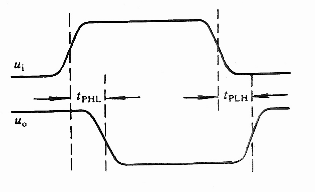
\includegraphics[width=3in]{H:/电子技术试验/4-18/4-18-3.png}
    \caption{延迟时间} \label{fig:aa}
\end{figure}




\section{\zihao{4} 实验电路}
\begin{figure}[h]
	\begin{minipage}[t]{0.5\linewidth} % 如果一行放2个图,用0.5,如果3个图,用0.33  
	  \centering   
	  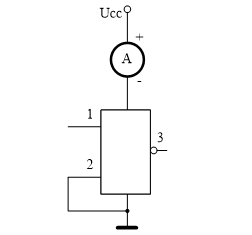
\includegraphics[width=2.2in]{H:/电子技术试验/4-18/4-18-4.png}   
	  \caption{$I_{EH}$}   
	  \label{fig:side:a}   
	\end{minipage}%   
	\begin{minipage}[t]{0.5\linewidth}   
	  \centering   
	  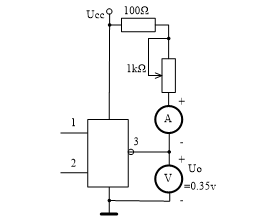
\includegraphics[width=2.8in]{H:/电子技术试验/4-18/4-18-5.png}   
	  \caption{$N_o$}   
	  \label{fig:side:b}   
	\end{minipage}   
  \end{figure}
  \begin{figure}[h]
	\begin{minipage}[t]{0.5\linewidth} % 如果一行放2个图,用0.5,如果3个图,用0.33  
	  \centering   
	  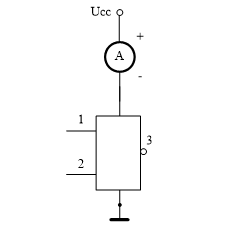
\includegraphics[width=2.3in]{H:/电子技术试验/4-18/4-18-6.png}   
	  \caption{$I_{EL}$}   
	  \label{fig:side:a}   
	\end{minipage}%   
	\begin{minipage}[t]{0.5\linewidth}   
	  \centering   
	  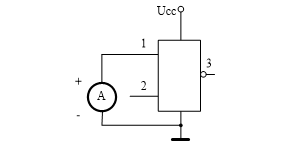
\includegraphics[width=2.9in]{H:/电子技术试验/4-18/4-18-7.png}   
	  \caption{$I_{IS}$}   
	  \label{fig:side:b}   
	\end{minipage}   
  \end{figure}
  \begin{figure}[h]
	\begin{minipage}[t]{0.5\linewidth} % 如果一行放2个图,用0.5,如果3个图,用0.33  
	  \centering   
	  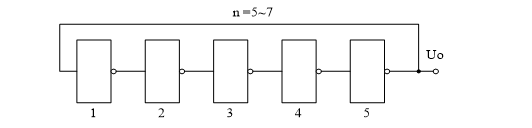
\includegraphics[width=4.3in]{H:/电子技术试验/4-18/4-18-8.png}   
	  \caption{$t_{pd}$}   
	  \label{fig:side:a}   
	\end{minipage}%   
	\begin{minipage}[t]{0.5\linewidth}   
	  \centering   
	  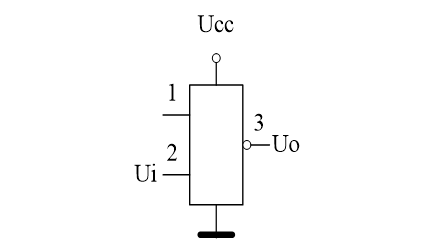
\includegraphics[width=3in]{H:/电子技术试验/4-18/4-18-9.png}   
	  \caption{电压传输特性}   
	  \label{fig:side:b}   
	\end{minipage}   
  \end{figure}


  \newpage
\section{\zihao{4} 实验内容及步骤}
(1)按表1验证74LS00的逻辑功能\par
(2)分别按图4、图6、图7、图5、图8接线,测出与非门      
的主要参数$I_{EH}$、$I_{EL}$、$I_{IS}$、$N_o$、$t_{pd}$,并将结果填入表2中。\par
(3)按图9的方法测试与非门的电压传输特性。$U_i$为三角波,f=1kHz,幅度
$U_p=5(v)$。\par
 
\newpage


\section{\zihao{4} 数据及误差处理}
\subsection{74LS00的逻辑功能}
\begin{table}[h]
    \centering  
    \begin{tabular}{c|c|c|c}
        \hline
        \multicolumn{2}{c}{输入端} \vline  &  \multicolumn{2}{c}{输出端} \vline \\ \hline
              k1            & k2           &  LED指示          &  电压表测量值 \\ \hline
              0             & 0            &   H               &  3.511V             \\ \hline
              0             & 1            &   H               &  3.510V          \\ \hline
              1             & 0            &   H               &   3.510V     \\ \hline
              1             & 1            &   L               &   0.136V     \\ \hline
    \end{tabular}
  \end{table}




\subsection{74LS00的主要参数}
\begin{table}[h]
    \centering  
    \begin{tabular}{c|c|c|c|c|c}
        \hline
           与非门主要参数    & $I_{EL}$         & $I_{EH}$    & $I_{IS}$   &  $N_o$  &  $t_{pd}$ \\ \hline
              测量值         & 2.585mA          &  2.440mA    &   0.224mA  &  49.17     & 6.61ns      \\ \hline
        \end{tabular}
\end{table}
\[N_o=\frac{I_{oLmax}}{I_{IS}}=49.17\]

\[t_{pd}\approx \frac{T}{2N}=\frac{1}{2Nf}=6.61ns \]

空载导通功耗$P_L$:
             \[P_L=I_{EL}\times U_{CC}=12.93mW\]
空载截止功率$P_H$:
             \[P_H=I_{EH}\times U_{CC}=12.20mW\]
则其平均功耗为
             \[P=\frac{P_L+P_H}{2}=12.57mW\]


             \newpage

\subsection{74LS00的电压传输特性}
测量图
\begin{figure}[h]
    %\small
    \centering
    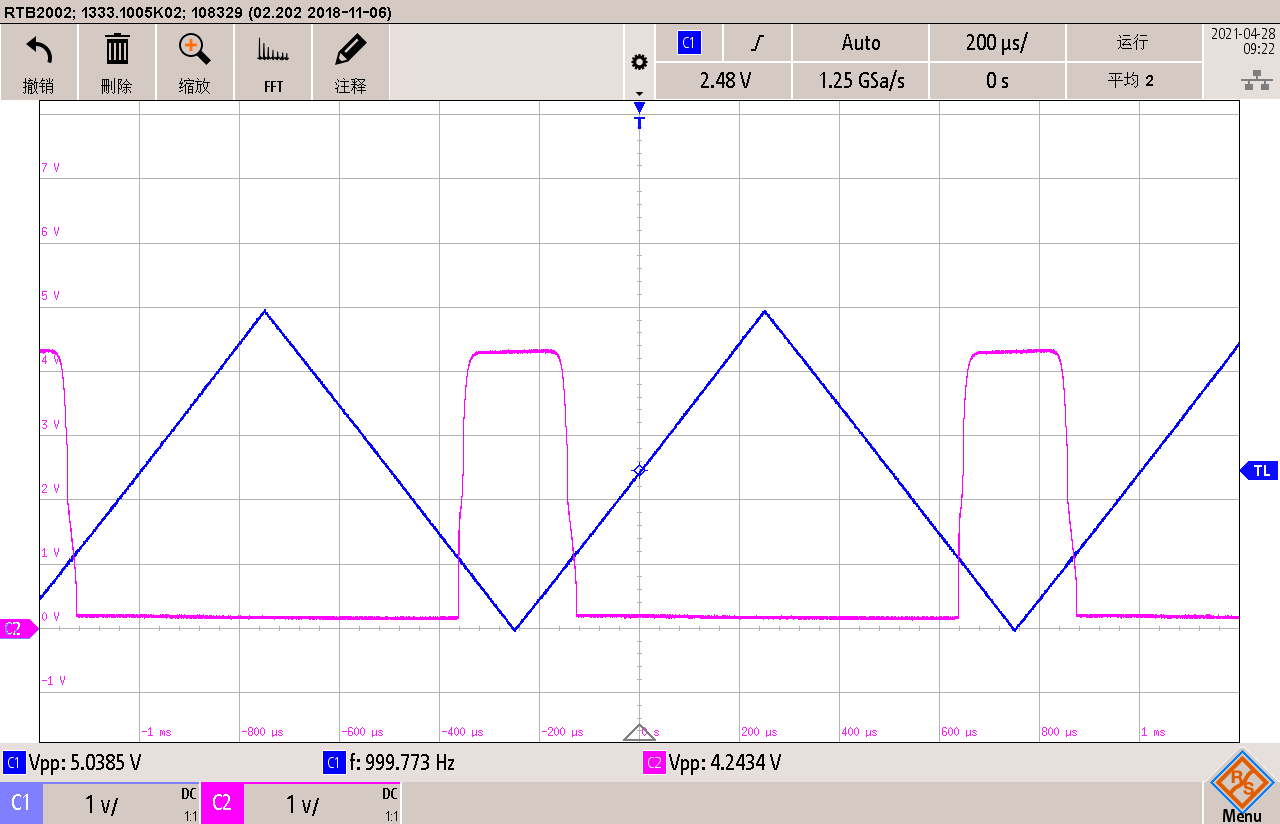
\includegraphics[width=4.2in]{H:/电子技术试验/4-18/4-18-12.png}
    \caption{输入与输出电压} \label{fig:aa}
\end{figure}
\begin{figure}[h]
    %\small
    \centering
    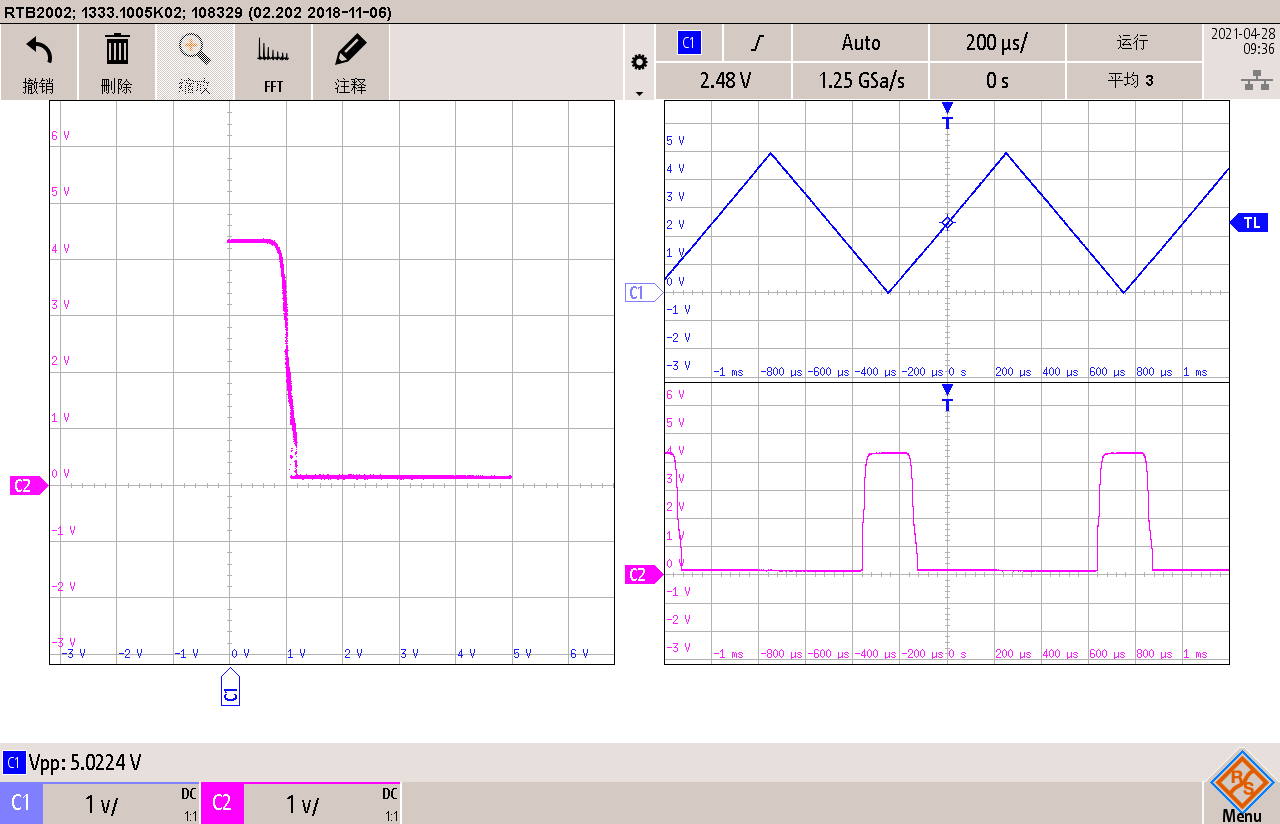
\includegraphics[width=4.2in]{H:/电子技术试验/4-18/4-18-11.png}
    \caption{电压传输特性} \label{fig:aa}
\end{figure}

\newpage
  理论值:
  \begin{figure}[h]
    %\small
    \centering
    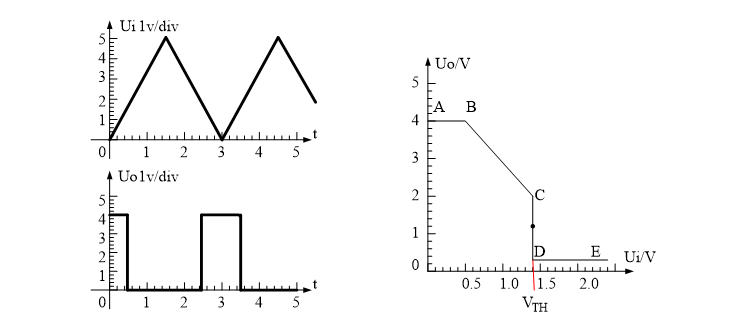
\includegraphics[width=5in]{H:/电子技术试验/4-18/4-18-10.png}
    \caption{延迟时间} \label{fig:aa}
\end{figure}

  \begin{table}[h]
    \centering  
    \begin{tabular}{c|c|c|c}
        \hline
         相关参数    & $U_{oH}$         & $U_{oL}$    & $U_{TH}$       \\ \hline
           测量值    & 4.32V             & 0.17V         &    1.2V                 \\ \hline
    \end{tabular}
\end{table}



	\section{\zihao{4} 实验设备和器材}
	(1)双踪示波器             \qquad \qquad \qquad \qquad \qquad  \qquad           1台\par
	(2)直流稳压电源             \qquad \quad \qquad \qquad \qquad \qquad           1台\par
	(3)数字逻辑实验箱            \qquad  \qquad \qquad \qquad\qquad                1台\par
	(4)万用表                   \qquad  \qquad \qquad \qquad \qquad \qquad \qquad  1只\par
	(5)集成四-2输入与非门(74LS00) \qquad    \quad                                    2片\par
    (6)函数发生器          \qquad  \qquad  \qquad \qquad \qquad\qquad                1台\par
	(7)电阻                 \quad    \qquad  \qquad \qquad \qquad \qquad \qquad \qquad  1只\par
    (8)多圈电位器                  \qquad \qquad \qquad \qquad \qquad \qquad  1只\par

\section{结论}
(1)逻辑与非门满足逻辑关系Y=(AB)'\par 
(2)逻辑与非门器件74LS00的平均功耗约为12.5mW左右,其输入短路电流较小,输入短路电流越小,带负载数量越大,即扇出系数越大。\par
(3)电压传输特性,在转折区,与非门的输出电压会发生急剧变化,转折中点阈值电压测量值约为   ,和通常值有一定差别,这是芯片自身的差异造成的。
\par
\newpage
\section{思考}
(1)门电路的带负载能力是什么?\par 
带负载能力就是代表器件的输出电流的大小。对于标准TTL器件,指上级负载能够外接器件,同时输出的电压或电流大小不受影响的能力。\par

(2)测量扇出系数 $N_o$的原理是什么?\par

扇出系数 $N_o$是指输出端最多能带同类门的个数。它反映门电路输出端驱动负载的能力。 \[N_o=\frac{I_{oLmax}}{I_{IS}}\]
式中$I_{oLmax}$在$U_{oL}$不大于0.35V时允许灌入输入端的最大灌入负载电流;
$I_s$是TTL 逻辑 门的输入短路电流,实验通过调节如图5中电位器$ R_L$,的阻值,使输出电压$U_o=0.35V$,测出此时的负载电流 $I_{oLmax}$,这就是允许灌入的最大负载电流。
\par 
(3)在什么情况下与非门可以输出高电平或低电平?其电压值分别约为多少?\par 
输入电平在传输特性的转折区之前可以输出高电平,在转折区之后可以输出低电平。电压值分别大约为3.51V和0.136V
\par
(4)与非门多余输入端应如何处理?\par
与非门多于的输入端置为1则不影响结果
至于多余输入端的处理原则,应该使其值不能影响逻辑器件的正常功能\par
\end{document}